% Options for packages loaded elsewhere
\PassOptionsToPackage{unicode}{hyperref}
\PassOptionsToPackage{hyphens}{url}
%
\documentclass[
]{report}
\usepackage{lmodern}
\usepackage{amssymb,amsmath}
\usepackage{ifxetex,ifluatex}
\ifnum 0\ifxetex 1\fi\ifluatex 1\fi=0 % if pdftex
  \usepackage[T1]{fontenc}
  \usepackage[utf8]{inputenc}
  \usepackage{textcomp} % provide euro and other symbols
\else % if luatex or xetex
  \usepackage{unicode-math}
  \defaultfontfeatures{Scale=MatchLowercase}
  \defaultfontfeatures[\rmfamily]{Ligatures=TeX,Scale=1}
\fi
% Use upquote if available, for straight quotes in verbatim environments
\IfFileExists{upquote.sty}{\usepackage{upquote}}{}
\IfFileExists{microtype.sty}{% use microtype if available
  \usepackage[]{microtype}
  \UseMicrotypeSet[protrusion]{basicmath} % disable protrusion for tt fonts
}{}
\makeatletter
\@ifundefined{KOMAClassName}{% if non-KOMA class
  \IfFileExists{parskip.sty}{%
    \usepackage{parskip}
  }{% else
    \setlength{\parindent}{0pt}
    \setlength{\parskip}{6pt plus 2pt minus 1pt}}
}{% if KOMA class
  \KOMAoptions{parskip=half}}
\makeatother
\usepackage{xcolor}
\IfFileExists{xurl.sty}{\usepackage{xurl}}{} % add URL line breaks if available
\IfFileExists{bookmark.sty}{\usepackage{bookmark}}{\usepackage{hyperref}}
\hypersetup{
  pdftitle={  STAT 216 Activity Coursepack},
  hidelinks,
  pdfcreator={LaTeX via pandoc}}
\urlstyle{same} % disable monospaced font for URLs
\usepackage{color}
\usepackage{fancyvrb}
\newcommand{\VerbBar}{|}
\newcommand{\VERB}{\Verb[commandchars=\\\{\}]}
\DefineVerbatimEnvironment{Highlighting}{Verbatim}{commandchars=\\\{\}}
% Add ',fontsize=\small' for more characters per line
\usepackage{framed}
\definecolor{shadecolor}{RGB}{248,248,248}
\newenvironment{Shaded}{\begin{snugshade}}{\end{snugshade}}
\newcommand{\AlertTok}[1]{\textcolor[rgb]{0.94,0.16,0.16}{#1}}
\newcommand{\AnnotationTok}[1]{\textcolor[rgb]{0.56,0.35,0.01}{\textbf{\textit{#1}}}}
\newcommand{\AttributeTok}[1]{\textcolor[rgb]{0.77,0.63,0.00}{#1}}
\newcommand{\BaseNTok}[1]{\textcolor[rgb]{0.00,0.00,0.81}{#1}}
\newcommand{\BuiltInTok}[1]{#1}
\newcommand{\CharTok}[1]{\textcolor[rgb]{0.31,0.60,0.02}{#1}}
\newcommand{\CommentTok}[1]{\textcolor[rgb]{0.56,0.35,0.01}{\textit{#1}}}
\newcommand{\CommentVarTok}[1]{\textcolor[rgb]{0.56,0.35,0.01}{\textbf{\textit{#1}}}}
\newcommand{\ConstantTok}[1]{\textcolor[rgb]{0.00,0.00,0.00}{#1}}
\newcommand{\ControlFlowTok}[1]{\textcolor[rgb]{0.13,0.29,0.53}{\textbf{#1}}}
\newcommand{\DataTypeTok}[1]{\textcolor[rgb]{0.13,0.29,0.53}{#1}}
\newcommand{\DecValTok}[1]{\textcolor[rgb]{0.00,0.00,0.81}{#1}}
\newcommand{\DocumentationTok}[1]{\textcolor[rgb]{0.56,0.35,0.01}{\textbf{\textit{#1}}}}
\newcommand{\ErrorTok}[1]{\textcolor[rgb]{0.64,0.00,0.00}{\textbf{#1}}}
\newcommand{\ExtensionTok}[1]{#1}
\newcommand{\FloatTok}[1]{\textcolor[rgb]{0.00,0.00,0.81}{#1}}
\newcommand{\FunctionTok}[1]{\textcolor[rgb]{0.00,0.00,0.00}{#1}}
\newcommand{\ImportTok}[1]{#1}
\newcommand{\InformationTok}[1]{\textcolor[rgb]{0.56,0.35,0.01}{\textbf{\textit{#1}}}}
\newcommand{\KeywordTok}[1]{\textcolor[rgb]{0.13,0.29,0.53}{\textbf{#1}}}
\newcommand{\NormalTok}[1]{#1}
\newcommand{\OperatorTok}[1]{\textcolor[rgb]{0.81,0.36,0.00}{\textbf{#1}}}
\newcommand{\OtherTok}[1]{\textcolor[rgb]{0.56,0.35,0.01}{#1}}
\newcommand{\PreprocessorTok}[1]{\textcolor[rgb]{0.56,0.35,0.01}{\textit{#1}}}
\newcommand{\RegionMarkerTok}[1]{#1}
\newcommand{\SpecialCharTok}[1]{\textcolor[rgb]{0.00,0.00,0.00}{#1}}
\newcommand{\SpecialStringTok}[1]{\textcolor[rgb]{0.31,0.60,0.02}{#1}}
\newcommand{\StringTok}[1]{\textcolor[rgb]{0.31,0.60,0.02}{#1}}
\newcommand{\VariableTok}[1]{\textcolor[rgb]{0.00,0.00,0.00}{#1}}
\newcommand{\VerbatimStringTok}[1]{\textcolor[rgb]{0.31,0.60,0.02}{#1}}
\newcommand{\WarningTok}[1]{\textcolor[rgb]{0.56,0.35,0.01}{\textbf{\textit{#1}}}}
\usepackage{longtable,booktabs}
% Correct order of tables after \paragraph or \subparagraph
\usepackage{etoolbox}
\makeatletter
\patchcmd\longtable{\par}{\if@noskipsec\mbox{}\fi\par}{}{}
\makeatother
% Allow footnotes in longtable head/foot
\IfFileExists{footnotehyper.sty}{\usepackage{footnotehyper}}{\usepackage{footnote}}
\makesavenoteenv{longtable}
\usepackage{graphicx}
\makeatletter
\def\maxwidth{\ifdim\Gin@nat@width>\linewidth\linewidth\else\Gin@nat@width\fi}
\def\maxheight{\ifdim\Gin@nat@height>\textheight\textheight\else\Gin@nat@height\fi}
\makeatother
% Scale images if necessary, so that they will not overflow the page
% margins by default, and it is still possible to overwrite the defaults
% using explicit options in \includegraphics[width, height, ...]{}
\setkeys{Gin}{width=\maxwidth,height=\maxheight,keepaspectratio}
% Set default figure placement to htbp
\makeatletter
\def\fps@figure{htbp}
\makeatother
\setlength{\emergencystretch}{3em} % prevent overfull lines
\providecommand{\tightlist}{%
  \setlength{\itemsep}{0pt}\setlength{\parskip}{0pt}}
\setcounter{secnumdepth}{-\maxdimen} % remove section numbering
\usepackage{booktabs}
\usepackage{geometry}
\usepackage[none]{hyphenat}

\pagestyle{plain}

%%%% Set margins?... doesn't work
\setlength{\topmargin}{-1cm}
\addtolength{\evensidemargin}{-1cm}
\addtolength{\oddsidemargin}{-1cm}
\addtolength{\textheight}{1.8cm}
\addtolength{\textwidth}{2cm}
\ifluatex
  \usepackage{selnolig}  % disable illegal ligatures
\fi
\usepackage[]{natbib}
\bibliographystyle{plainnat}

\title{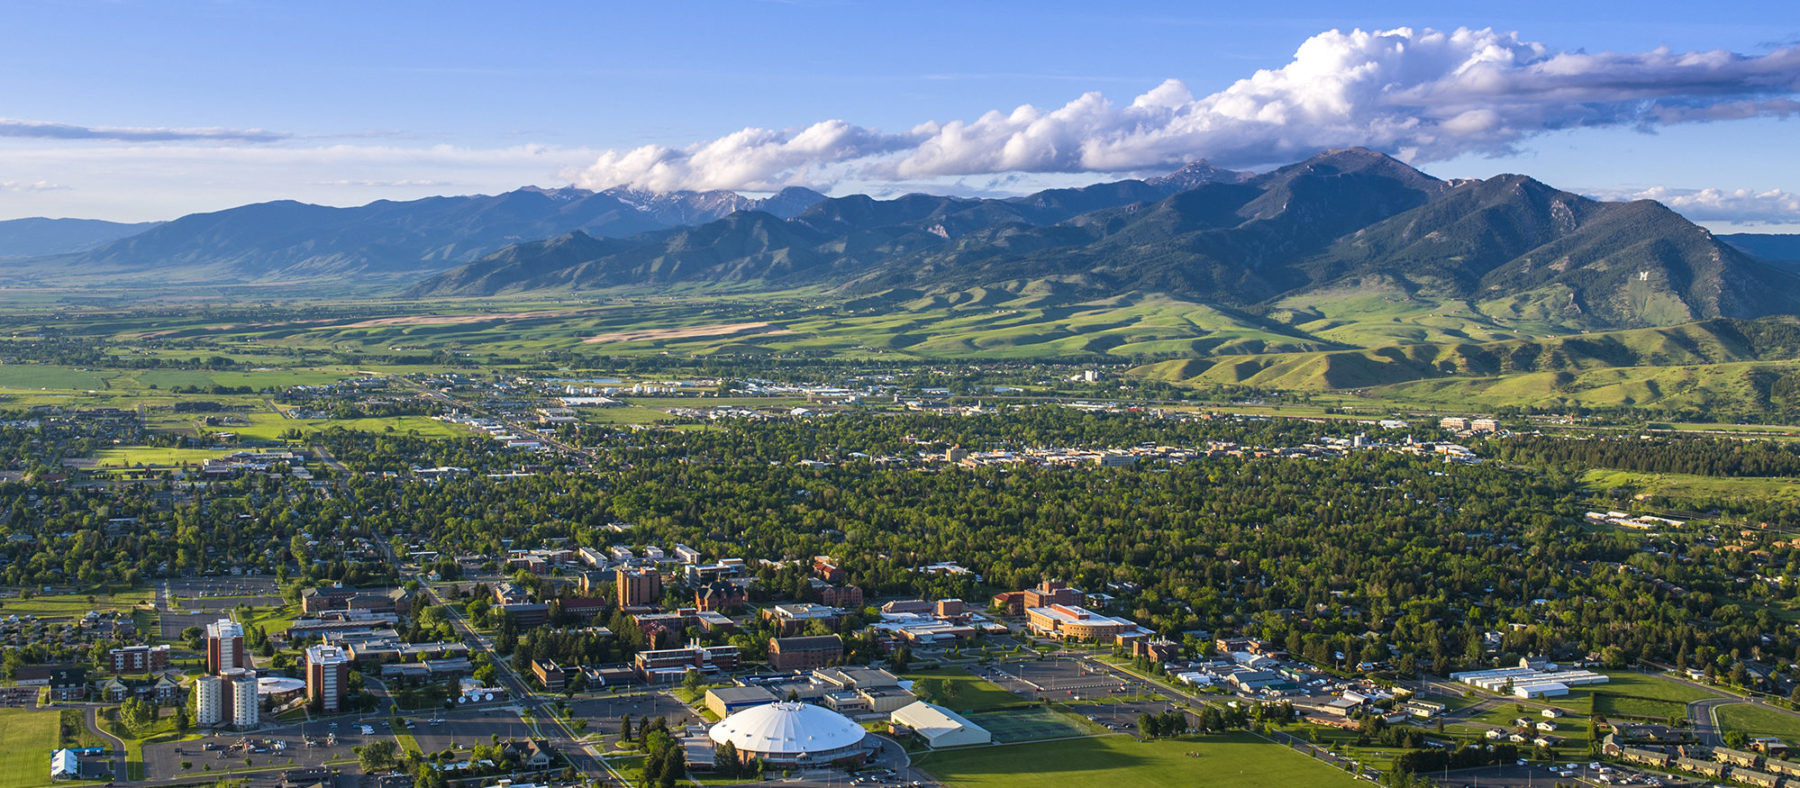
\includegraphics[width=5in,height=\textheight]{images/msu-campus.jpg}
\vspace{1cm}\\
STAT 216 Activity Coursepack}
\usepackage{etoolbox}
\makeatletter
\providecommand{\subtitle}[1]{% add subtitle to \maketitle
  \apptocmd{\@title}{\par {\large #1 \par}}{}{}
}
\makeatother
\subtitle{Fall 2020}
\author{}
\date{\vspace{-2.5em}}

\begin{document}
\maketitle

{
\setcounter{tocdepth}{0}
\tableofcontents
}
\hypertarget{preface}{%
\chapter{Preface}\label{preface}}

This coursepack accompanies the textbook for STAT 216: Introduction to Statistics at Montana State University. Each of the activities in this workbook is designed to target specific learning outcomes of the course, giving you practice with important statistical concepts in a group setting with instructor guidance. Bring this workbook with you to class each week, and take notes in the workbook as you would your own notes. A well-written complete workbook will provide an optimal study guide for exams!

\hypertarget{martian-alphabet}{%
\chapter{Martian Alphabet}\label{martian-alphabet}}

\hypertarget{learning-outcomes}{%
\section{Learning Outcomes}\label{learning-outcomes}}

\begin{itemize}
\item
  Describe the statistical investigation process
\item
  Identify observational units, variables, and variable types in a statistical study
\end{itemize}

\hypertarget{activity}{%
\section{Activity}\label{activity}}

How well can humans distinguish one ``Martian'' letter from another? In today's activity, we'll find out. When shown the two Martian letters, Kiki and Bumba, write down whether you think Bumba is on the left or the right.

\vspace{0.5in}

\hypertarget{steps-of-statistical-investigation}{%
\subsection{Steps of Statistical Investigation}\label{steps-of-statistical-investigation}}

The first step of any statistical investigation is to ask a research question. In this study the research question is: can we as a class read Martian? (we will refine this later on!). To answer any research question, we must design a study and collect data. (This will normally be provided for you in class.) For our question, the study consists of each student being presented with two Martian letters and asking which was Bumba. Your responses will become our observed data that we will explore. To answer the research question we will simulate what \emph{could} have happened in our class given random chance, repeat that many times to understand the expected variability between different ``randomly guessing'' classes, then comparing our class's observed data to the simulation. This gives us an estimate of how often (or the probability of) our class's result would occur if we were all merely guessing, allowing us to determine if we as a class can in fact read Martian.

Let's explore the data.
\textbf{Observational units} or \textbf{cases} are the subjects data is collected on. In a data set the rows will represent a single observational unit.

\begin{enumerate}
\def\labelenumi{\arabic{enumi}.}
\tightlist
\item
  What are the observational units in this study?
\end{enumerate}

\vspace{0.5in}

\begin{enumerate}
\def\labelenumi{\arabic{enumi}.}
\setcounter{enumi}{1}
\tightlist
\item
  How many students are in class today? This is the sample size.
\end{enumerate}

\vspace{0.5in}

\newpage

A \textbf{variable} is information collected or measured on each observational unit or case. We will look at two types of variables: \textbf{quantitative} and \textbf{categorical}. Each column in a data set will represent a different variable.

Quantitative variables are numerical measurements that can be discrete (whole, non-negative numbers) or continuous (any value within an interval). The number of students in a class would be a discrete variable as you can not have a partial student. GPA would be a continuous variable ranging from 0 to 4.0.

Categorical variables are data that are in groups or categories such as eye color, state of residency, or whether or not a student is considered in-state. Categorical variables with a natural ordering are considered ordinal variables while those without a natural ordering are considered a nominal variable. All variables will be treated as nominal for analysis.

\begin{figure}

{\centering 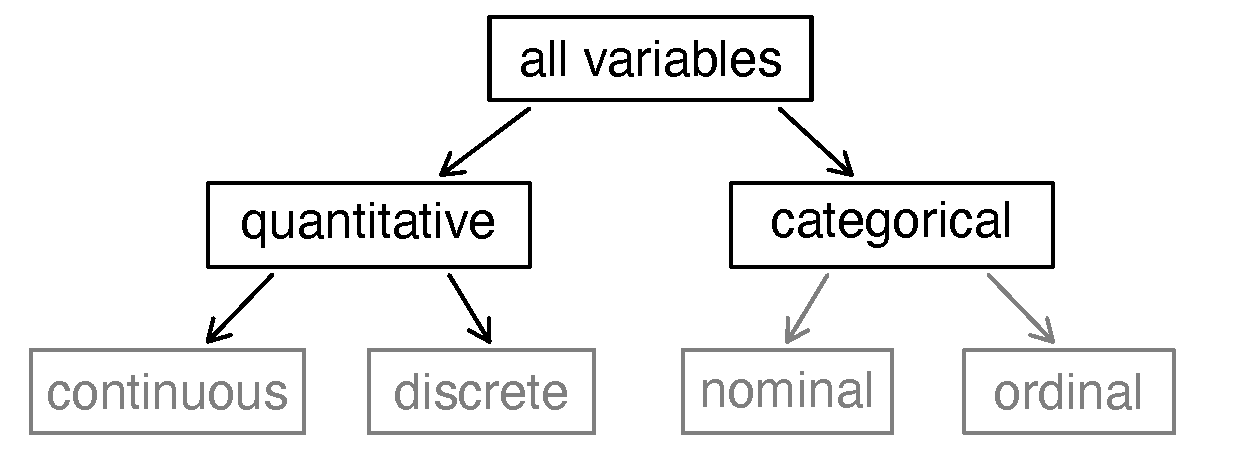
\includegraphics[width=0.75\linewidth]{images/variables} 

}

\caption{Types of variables.}\label{fig:unnamed-chunk-1}
\end{figure}

\begin{enumerate}
\def\labelenumi{\arabic{enumi}.}
\setcounter{enumi}{2}
\tightlist
\item
  Identify the variable we are collecting on each observational unit in this study, i.e., what are we measuring on each student?
\end{enumerate}

\vspace{.8in}

It is important to note that a variable is different than a summary statistic. A variable is measured on a \textbf{single observational unit} while a summary statistic is calculated from a group of observational units. For example, the variable \textbf{whether or not a student is considered in-state} can be measured on each individual student. In a class of 50 students we can calculate the proportion of students who are considered in-state, the summary statistic. Make sure you wrote the variable in question 3 as a variable \textbf{NOT} a summary statistic.

\begin{enumerate}
\def\labelenumi{\arabic{enumi}.}
\setcounter{enumi}{3}
\tightlist
\item
  Is the variable identified in question 3 categorical or quantitative?
\end{enumerate}

\vspace{0.3in}

\begin{enumerate}
\def\labelenumi{\arabic{enumi}.}
\setcounter{enumi}{4}
\tightlist
\item
  Were you correct or incorrect in identifying Bumba?
\end{enumerate}

\vspace{0.3in}

We will now collect the data from the entire class.

\begin{enumerate}
\def\labelenumi{\arabic{enumi}.}
\setcounter{enumi}{5}
\tightlist
\item
  How many people in your class were correct in identifying Bumba? Using the class size from question 2, calculate the proportion of students who correctly identified Bumba.
\end{enumerate}

\begin{center}
$\mbox{proportion} = \frac{\mbox{number of students who correctly identified Bumba}}{\mbox{total number of students}}$
\end{center}

\newpage

Looking at the data set and the summary statistics is only one way to display the data. We will also want to create a visualization or picture of the data. A \textbf{frequency bar plot} is used to display categorical data as a count or frequency. Since our variable has two levels, correct or incorrect, we will create two bars one for each level.

\begin{enumerate}
\def\labelenumi{\arabic{enumi}.}
\setcounter{enumi}{6}
\tightlist
\item
  Plot the observed class data using a frequency bar plot.
\end{enumerate}

\begin{flushleft}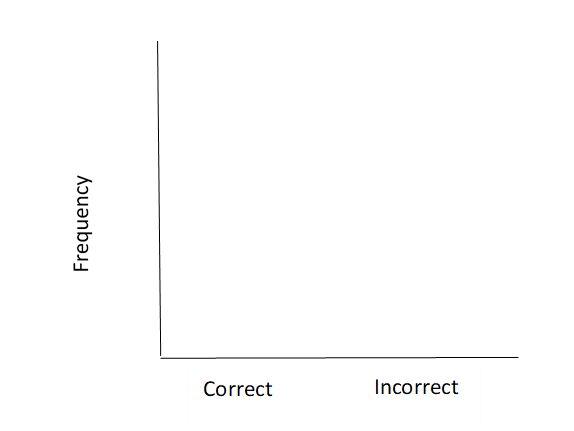
\includegraphics[width=0.75\linewidth]{images/barplot_martian} \end{flushleft}

We can also visualize the data as a proportion in a \textbf{relative frequency bar plot}. Relative frequency is the proportion calculated for each level of the categorical variable.

\begin{enumerate}
\def\labelenumi{\arabic{enumi}.}
\setcounter{enumi}{7}
\tightlist
\item
  Plot the observed class data using a relative frequency bar plot.
\end{enumerate}

\begin{flushleft}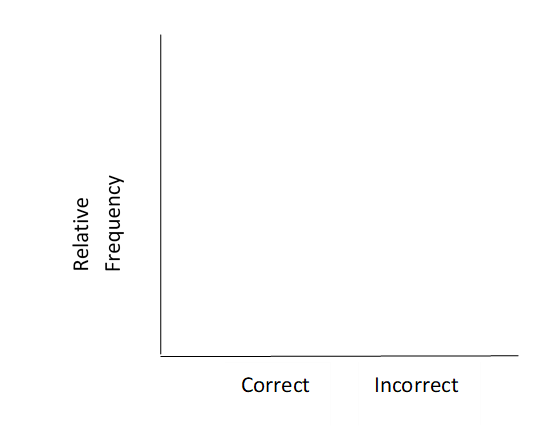
\includegraphics[width=0.75\linewidth]{images/relative_barplot_martian} \end{flushleft}

\newpage

\begin{enumerate}
\def\labelenumi{\arabic{enumi}.}
\setcounter{enumi}{8}
\item
  The next step is to analyze the data. If humans really don't know Martian and are just guessing which is Bumba, what are the chances of getting it right?
  \vspace{0.5in}

  How could we use a coin to simulate each student ``just guessing'' which martian letter is Bumba?
  \vspace{1in}

  How could we use coins to simulate the entire class ``just guessing'' which martian letter is Bumba?
  \vspace{1in}

  How many people in your class would you expect to choose Bumba correctly just by chance? Explain your reasoning.
  \vspace{1in}
\item
  Each of you will flip a coin one time to simulate your ``guess''. Let Heads = correct, Tails = incorrect. What was the result of your simulation?
  \vspace{.4in}

  What was the result from your class's simulation? What proportion of students ``guessed'' correctly in the simulation?
  \vspace{.4in}
\item
  If students really don't know Martian and are just guessing which is Bumba, which seems more unusual: the result from your class's \textbf{simulation} or the observed proportion of students in your class that were correct (this is your data from question 6)? Explain your reasoning.
\end{enumerate}

\newpage

\begin{enumerate}
\def\labelenumi{\arabic{enumi}.}
\setcounter{enumi}{11}
\tightlist
\item
  While your observed class data is likely far different from the simulated ``just-guessing'' class, comparing our class data to a single simulation does not seem to give enough information. The differences seen could just be due to that set of coin flips! Let's simulate another class. Each student should flip your coin again. What was the result from your class's second simulation? What proportion of students ``guessed'' correctly in the second simulation? Create a plot to compare the two simulated results with the observed class result.
\end{enumerate}

\vspace{1in}

\begin{enumerate}
\def\labelenumi{\arabic{enumi}.}
\setcounter{enumi}{12}
\tightlist
\item
  We still unfortunately only have a couple of simulations to compare our class data to. It would be much better to be able to see how our class compared to hundreds or thousands of ``just-guessing'' classes. Since we don't want to flip coins all class period, your instructor will use a computer simulation to get 1000 trials. Fill in the following blanks to describe how we would create a simulation of random guessing with 1000 trials.
\end{enumerate}

~~~~~~~~~~Probability of correct guesses: \_\_\_\_\_

\vspace{0.1in}

~~~~~~~~~~Sample size: \_\_\_\_\_

\vspace{0.1in}

~~~~~~~~~~Number of repetitions: \_\_\_\_\_

\vspace{0.1in}

\begin{enumerate}
\def\labelenumi{\arabic{enumi}.}
\setcounter{enumi}{13}
\tightlist
\item
  Sketch the distribution displayed by your instructor here, being sure to label each axis appropriately.
\end{enumerate}

\vspace{2in}

\begin{enumerate}
\def\labelenumi{\arabic{enumi}.}
\setcounter{enumi}{14}
\tightlist
\item
  Is your class particularly good or bad at Martian? How can you use the plot in question 14 to tell?
\end{enumerate}

\vspace{1in}

\begin{enumerate}
\def\labelenumi{\arabic{enumi}.}
\setcounter{enumi}{15}
\tightlist
\item
  Is it \emph{possible} that we could see our class results just by chance if everyone was just guessing? Explain your reasoning.
\end{enumerate}

\vspace{1in}

\begin{enumerate}
\def\labelenumi{\arabic{enumi}.}
\setcounter{enumi}{16}
\tightlist
\item
  Is it \emph{likely} that we could see our class results just by chance if everyone was just guessing? Explain your reasoning.
\end{enumerate}

\vspace{1in}

\begin{enumerate}
\def\labelenumi{\arabic{enumi}.}
\setcounter{enumi}{17}
\tightlist
\item
  Does this activity provide strong evidence that students were not just guessing at random? If so, what do you think is going on here? Can we as a class read Martian?
\end{enumerate}

\vspace{1in}

\hypertarget{take-home-messages}{%
\section{Take Home Messages}\label{take-home-messages}}

\begin{enumerate}
\def\labelenumi{\arabic{enumi}.}
\item
  In this course we will learn how to evaluate a claim by comparing observed results (classes' ``guesses'') to a distribution of many simulated results under an assumption like ``blind guessing.''
\item
  Blind guessing between two outcomes will be correct only about half the time. We can create data (via computer simulation) to fit the assumption of blind guessing.
\item
  Unusual observed results will make us doubt the assumptions used to create the simulated distribution. A large number of correct ``guesses'' is evidence that a person was not just blindly guessing.
\end{enumerate}

\hypertarget{additional-notes}{%
\section{Additional Notes}\label{additional-notes}}

Use this space to summarize your thoughts and take additional notes on today's activity, and to write down the names and contact information of your team mates.

\hypertarget{study-design}{%
\chapter{Study Design}\label{study-design}}

\hypertarget{learning-outcomes}{%
\section{Learning Outcomes}\label{learning-outcomes}}

\begin{itemize}
\item
  Explain the purpose of random sampling and its effect on scope of inference
\item
  Explain the purpose of random assignment and its effect on scope of inference
\item
  Identify whether a study is observational or an experiment
\item
  Identify confounding variables in observational studies and explain why they are confounding
\item
  Identify the types of bias present in a study
\end{itemize}

\hypertarget{terminology-review}{%
\section{Terminology Review}\label{terminology-review}}

Statistics is the study of how best to collect, analyze, and draw conclusions from data. Statistical inference will allow us to make a statement about a population parameter based on a sample statistic.

Some terms covered in this activity are\ldots{}

\begin{itemize}
\item
  Population
\item
  Sample
\item
  Parameter
\item
  Statistic
\item
  Selection Bias
\item
  Response Bias
\item
  Non-response Bias
\item
  Scope of Inference
\item
  Explanatory Variable
\item
  Response Variable
\item
  Confounding Variable
\item
  Experiments
\item
  Observational Study
\end{itemize}

To review these concepts see Section 1.3 to 1.6 in the textbook.

\newpage

\hypertarget{types-of-bias}{%
\section{Types of Bias}\label{types-of-bias}}

There are two parts to study design: how the sample was selected and how the study was conducted. First we will look at sampling and types of bias.

In these next questions, identify the target population, the sample, the variable, and the type of bias present.

\begin{enumerate}
\def\labelenumi{\arabic{enumi}.}
\item
  To determine if the proportion of out of state undergraduate students at Montana State University has increased in the last 10 years, a statistics instructor sent an email survey to 500 randomly selected current undergraduate students. One of the questions on the survey asked whether they had in-state or out-of-state residency. She only received 378 responses.
  \vspace{0.25in}

  Target population:
  \vspace{0.3in}

  Sample:
  \vspace{0.3in}

  Variable:
  \vspace{0.3in}

  Type of Bias:
  \vspace{0.3in}
\item
  PEW Research surveys US adults about many different topics. Recently a survey was conducted to assess current presidential approval. A random sample of 6395 US adults was taken. Of those surveyed, 42\% say they agree with President Trump on many or nearly all of the top issues facing the country today.
  \vspace{0.25in}

  Target population:
  \vspace{0.3in}

  Sample:
  \vspace{0.3in}

  Variable:
  \vspace{0.3in}

  Type of Bias:
  \vspace{0.3in}
\end{enumerate}

\newpage

\begin{enumerate}
\def\labelenumi{\arabic{enumi}.}
\setcounter{enumi}{2}
\item
  A television station is interested in predicting whether or not voters in its listening area are opposed to legalizing marijuana for adult use. It asks its viewers to phone in and indicate whether they are in favor of this or opposed to this. Of the 2241 viewers who phoned in, forty-five percent were opposed to legalizing marijuana.
  \vspace{0.1in}

  Target population:
  \vspace{0.3in}

  Sample:
  \vspace{0.3in}

  Variable:
  \vspace{0.3in}

  Type of Bias:
  \vspace{0.3in}
\item
  To gauge the interest in a new swimming pool, a local organization stood outside of the Bogart Pool during open hours. One of the questions they asked was, ``Since the Bogart Pool is in such bad repair, don't you agree that the city should fund a new pool?''
  \vspace{0.1in}

  Target population:
  \vspace{0.3in}

  Sample:
  \vspace{0.3in}

  Variable:
  \vspace{0.3in}

  Type of Bias:
  \vspace{0.3in}
\item
  The Bozeman school district is interested in surveying parents of students about their opinions on returning to school this fall following the COVID-19 pandemic. They divided the school district into 10 divisions based on location and randomly surveyed 20 households within each division.
  \vspace{0.1in}

  Target population:
  \vspace{0.3in}

  Sample:
  \vspace{0.3in}

  Variable:
  \vspace{0.3in}

  Type of Bias:
  \vspace{0.3in}
\end{enumerate}

\newpage

\hypertarget{study-design-1}{%
\section{Study Design}\label{study-design-1}}

The two main study designs we will cover are observational studies and experiments. Both the sampling method and the study design will help to determine the \textbf{scope of inference} for a study. Remember that only in a randomized experiment can we conclude a \textbf{causal} (cause and effect) relationship between the explanatory and response variable.

\begin{center}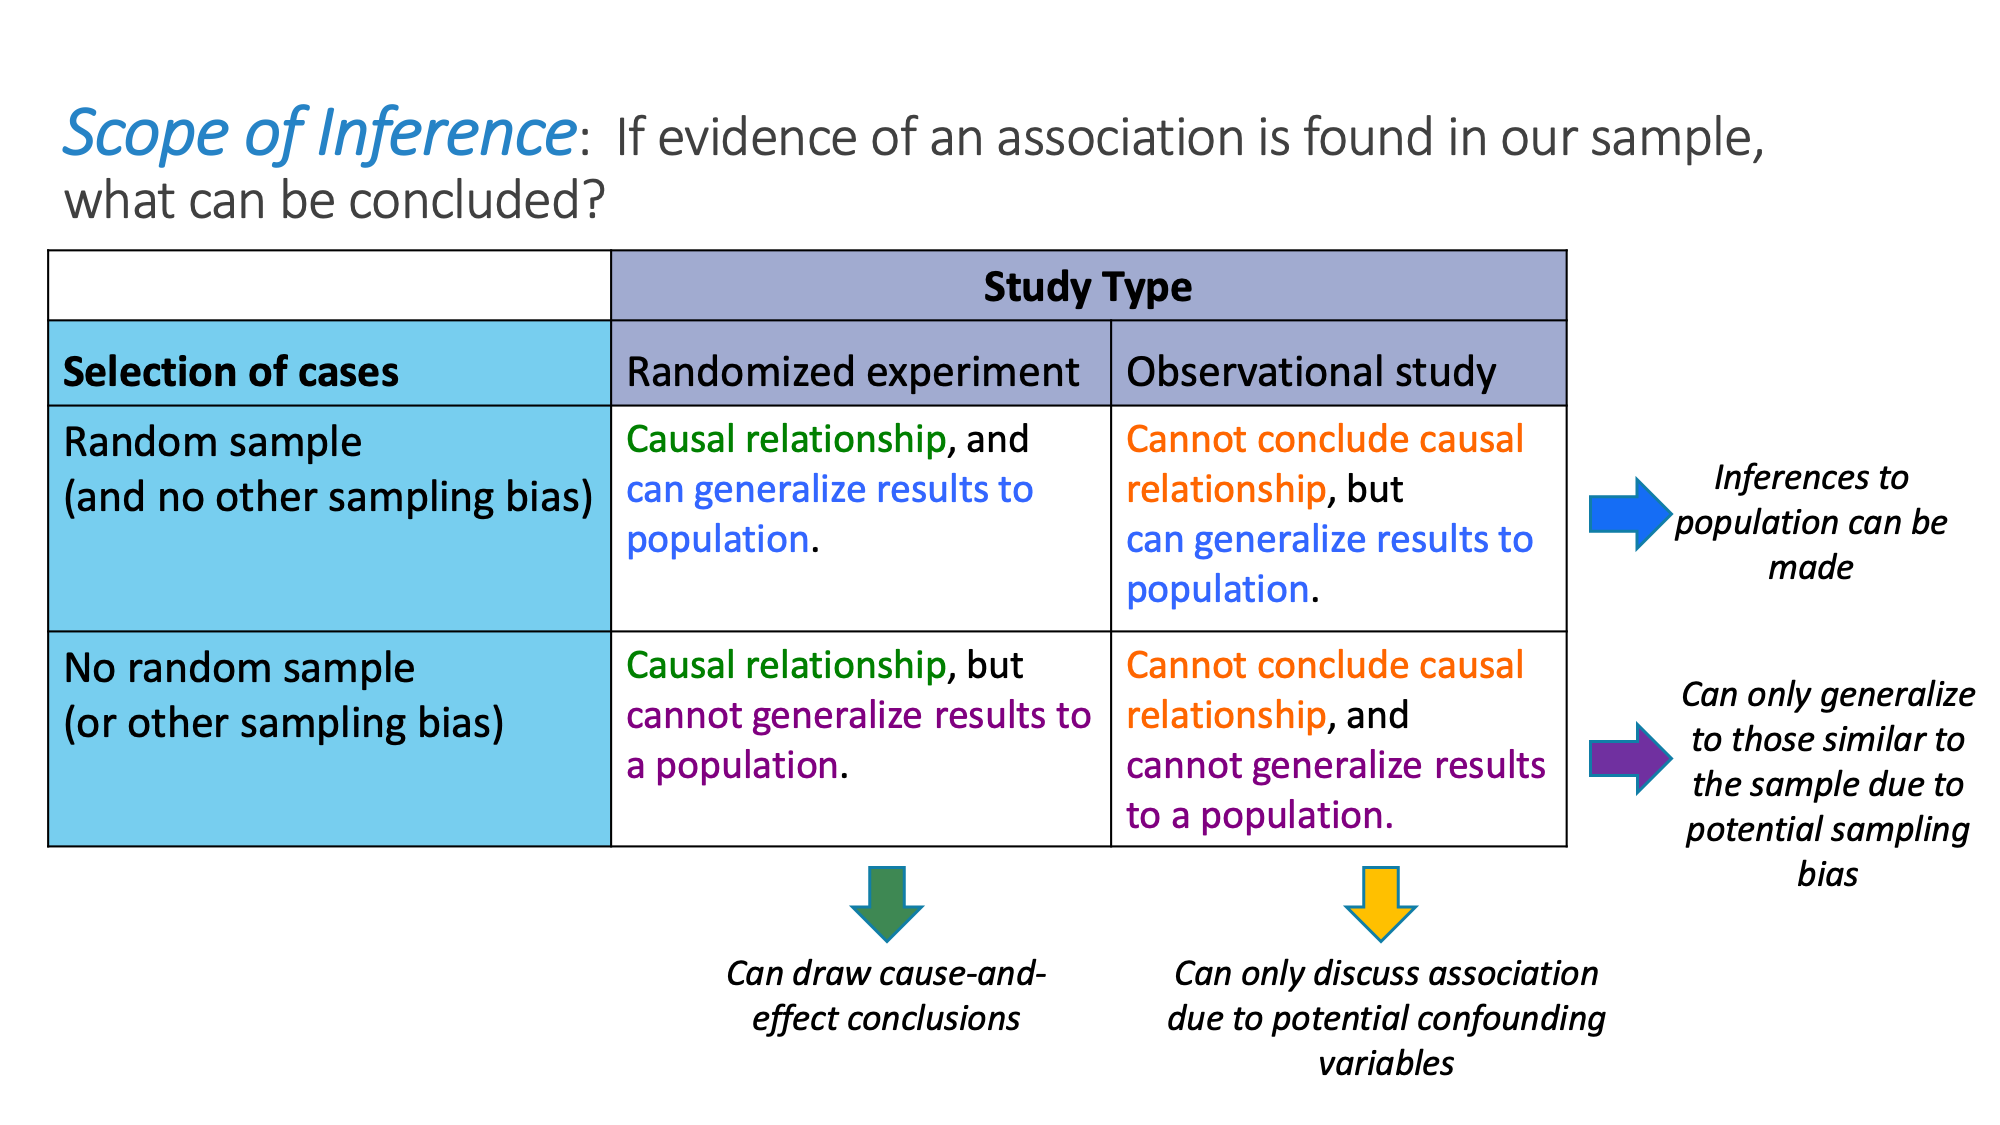
\includegraphics[width=0.75\linewidth]{images/ScopeOfInference} \end{center}

For the next exercises, identify the explanatory variable, the response variable, a potential confounding variable, and the study design.

\begin{enumerate}
\def\labelenumi{\arabic{enumi}.}
\setcounter{enumi}{5}
\item
  The pharmaceutical company, Moderna Therapeutics is working in conjunction with the National Institute of Health towards a vaccine for COVID-19 and has recently begun Phase 3 clinical trials. US Clinical research sites will enroll 30,000 volunteers without COVID-19 to participate. Participants will be randomly assigned to receive either the candidate vaccine or a saline placebo. They will then be followed to assess vaccine related symptoms and development of COVID-19. The trial is blinded, so the investigators and the participants will not know who is assigned to which group.
  \vspace{0.25in}

  Explanatory Variable:
  \vspace{0.25in}

  Response Variable:
  \vspace{0.25in}

  Confounding Variable:
  \vspace{0.25in}

  Study design:
  \vspace{0.25in}

  What is the scope of inference for this study?
  \vspace{0.5in}
\item
  In another study, a local health department randomly selected 1000 US adults without COVID-19 to participate in a health survey. Each participant was assessed at the beginning of the study and then followed for 1 year. They were interested to see which participants elected to receive a vaccination for COVID-19 and whether any participants developed COVID-19.
  \vspace{0.25in}

  Explanatory Variable:
  \vspace{0.25in}

  Response Variable:
  \vspace{0.25in}

  Confounding Variable:
  \vspace{0.25in}

  Study design:
  \vspace{0.25in}

  What is the scope of inference for this study?
  \vspace{0.5in}
\item
  What is a potential confounding variable for the study in question 7? Explain how this meets the definition of a confounding variable.
  \vspace{1in}
\end{enumerate}

\hypertarget{additional-notes}{%
\section{Additional Notes}\label{additional-notes}}

Use this space to summarize your thoughts and take additional notes on today's activity

\hypertarget{exploratory-data-analysis-categorical-variables}{%
\chapter{Exploratory Data Analysis: Categorical Variables}\label{exploratory-data-analysis-categorical-variables}}

\hypertarget{learning-outcomes}{%
\section{Learning Outcomes}\label{learning-outcomes}}

\begin{itemize}
\item
  Identify and create appropriate summary statistics and plots
  given a data set or research question
\item
  Plots for a single categorical variable: bar plot
\item
  Plots for association between two categorical variables:
  segmented bar plot, mosaic plot
\item
  Recognize and simulate probabilities as long-run frequencies
\item
  Construct two-way tables to evaluate conditional probabilities
\end{itemize}

\hypertarget{terminology-review}{%
\section{Terminology Review}\label{terminology-review}}

In today's activity we will review summary measures and plots for categorical variables. Some terms covered in this activity are\ldots{}

\begin{itemize}
\item
  Proportions
\item
  Bar plots
\item
  Segmented bar plots
\item
  Probability
\item
  Conditional Probability
\item
  Two-way tables
\end{itemize}

To review these concepts see Section 2.1 in the textbook.

\newpage

\hypertarget{activity}{%
\section{Activity}\label{activity}}

The data set we will use for this activity is from the Current Population Survey in 1985. The CPS is a survey sponsored by the Census Bureau and the Bureau of Labor Statistics to track labor force statistics for the United States population. The following table summarizes the data:

\begin{center}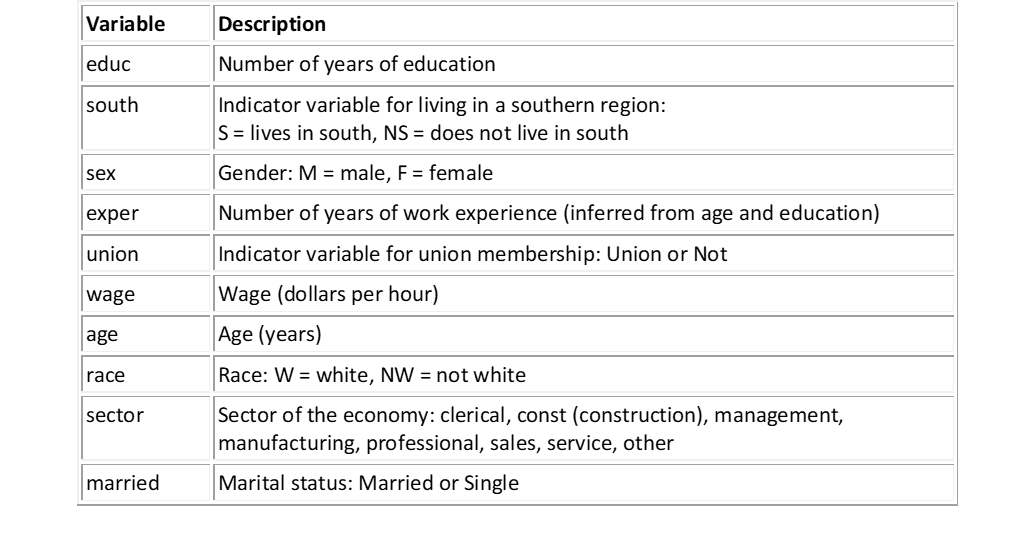
\includegraphics[width=0.7\linewidth]{images/cps} \end{center}

\hypertarget{vocabulary-review}{%
\subsection{Vocabulary Review}\label{vocabulary-review}}

\begin{enumerate}
\def\labelenumi{\arabic{enumi}.}
\tightlist
\item
  What are the observational units?
\end{enumerate}

\vspace{0.5in}

\begin{enumerate}
\def\labelenumi{\arabic{enumi}.}
\setcounter{enumi}{1}
\tightlist
\item
  Which variables are categorical?
\end{enumerate}

\vspace{0.5in}

\begin{enumerate}
\def\labelenumi{\arabic{enumi}.}
\setcounter{enumi}{2}
\tightlist
\item
  What types of plots can be used to display categorical data?
\end{enumerate}

\vspace{0.5in}

An important part of understanding data is to create visual pictures of what the data represents. In this activity we will create graphical representations of categorical data.

\hypertarget{displaying-a-single-categorical-variable.}{%
\subsection{Displaying a single categorical variable.}\label{displaying-a-single-categorical-variable.}}

If we wanted to know how many people in our data set were in each sector, we would create a bar plot of the variable sector.

\begin{center}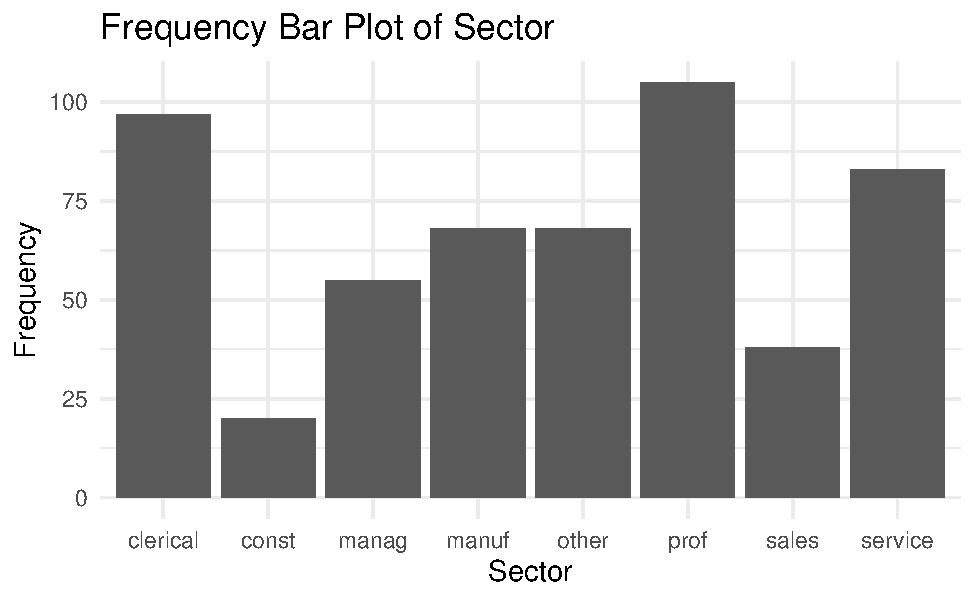
\includegraphics[width=0.7\linewidth]{03-EDA-categorical_files/figure-latex/unnamed-chunk-3-1} \end{center}

\begin{enumerate}
\def\labelenumi{\arabic{enumi}.}
\setcounter{enumi}{3}
\tightlist
\item
  Which Sector has the largest number of people in it?
\end{enumerate}

\vspace{0.5in}

We could also choose to display the data as a proportion in a relative frequency bar plot. To find the relative frequency divide the count in each sector by the sample size. These are sample proportions.

\begin{center}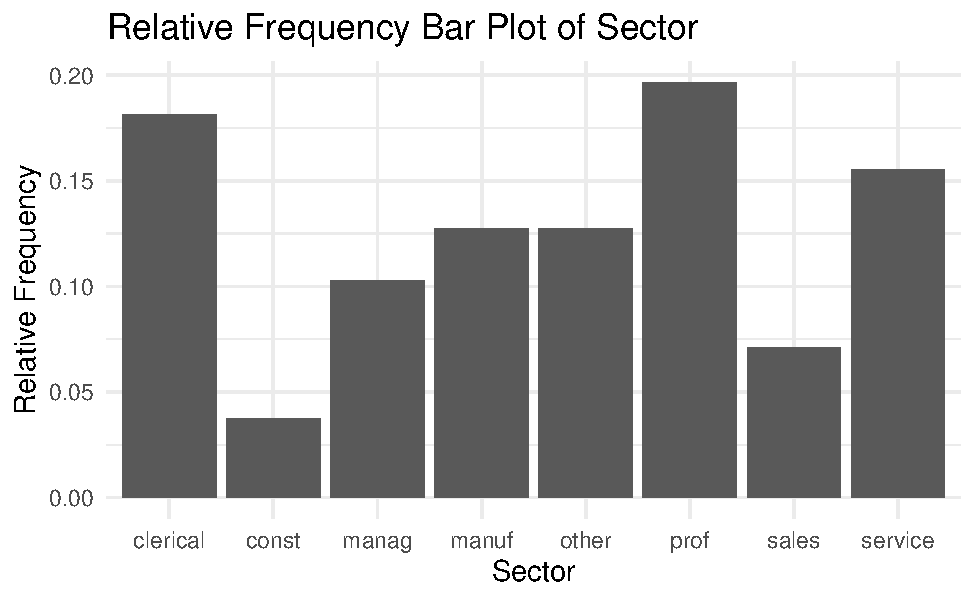
\includegraphics[width=0.7\linewidth]{03-EDA-categorical_files/figure-latex/unnamed-chunk-4-1} \end{center}

\begin{enumerate}
\def\labelenumi{\arabic{enumi}.}
\setcounter{enumi}{4}
\tightlist
\item
  What features in this plot are same as the frequency bar plot? Which are different?
\end{enumerate}

\newpage

\hypertarget{displaying-two-categorical-variables}{%
\subsection{Displaying two categorical variables}\label{displaying-two-categorical-variables}}

To see the differences in proportion of each sector between males and females we would create a segmented bar plot of sector segmented by sex.

\begin{center}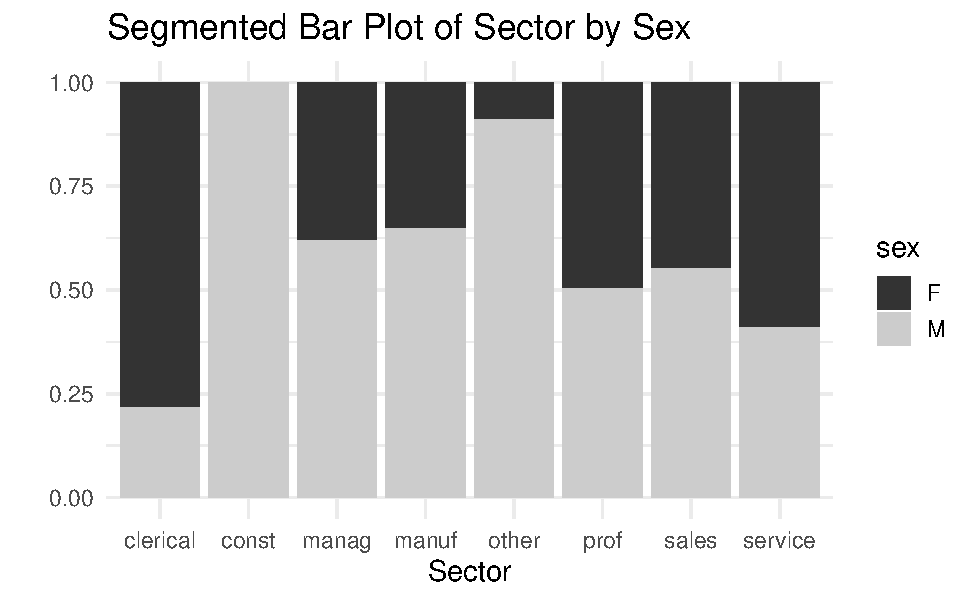
\includegraphics[width=0.7\linewidth]{03-EDA-categorical_files/figure-latex/unnamed-chunk-5-1} \end{center}

\begin{enumerate}
\def\labelenumi{\arabic{enumi}.}
\setcounter{enumi}{5}
\tightlist
\item
  Using the segmented bar plot, which sector has about the same proportion of males and females?
\end{enumerate}

\vspace{0.5in}

\begin{enumerate}
\def\labelenumi{\arabic{enumi}.}
\setcounter{enumi}{6}
\tightlist
\item
  Which sector has the highest proportion of females?
\end{enumerate}

\vspace{0.5in}

\begin{enumerate}
\def\labelenumi{\arabic{enumi}.}
\setcounter{enumi}{7}
\tightlist
\item
  Which variable is the explanatory variable? Which is the response variable?
\end{enumerate}

\newpage

\hypertarget{probability}{%
\section{Probability}\label{probability}}

\begin{enumerate}
\def\labelenumi{\arabic{enumi}.}
\setcounter{enumi}{8}
\tightlist
\item
  A study was reported in which ninth grade Minnesota teens were asked whether they had gambled at least once a week in the past year. The sample consisted of 49.1\% boys. The proportion of boys who had gambled at least once per week during the past year was 0.229, while among non-boys this proportion was only 0.045.\\
  Let B = the event the person is a boy, and C = the event the person is a weekly gambler.
  \vspace{0.1in}
\end{enumerate}

\begin{enumerate}
\def\labelenumi{\alph{enumi}.}
\item
  Draw a segmented bar plot of gambling segmented by sex.
  \vspace{2in}
\item
  Identify what each numerical value represents in probability notation.
  \vspace{.1in}
\end{enumerate}

~~~~~~~~~~~~~~~~0.491 = \vspace{.2in}\\
\hspace*{0.333em}\hspace*{0.333em}\hspace*{0.333em}\hspace*{0.333em}\hspace*{0.333em}\hspace*{0.333em}\hspace*{0.333em}\hspace*{0.333em}\hspace*{0.333em}\hspace*{0.333em}\hspace*{0.333em}\hspace*{0.333em}\hspace*{0.333em}\hspace*{0.333em}\hspace*{0.333em}\hspace*{0.333em}0.229 =

\vspace{.2in}

~~~~~~~~~~~~~~~~0.045 =

\vspace{.2in}

\begin{enumerate}
\def\labelenumi{\alph{enumi}.}
\setcounter{enumi}{2}
\tightlist
\item
  Create a two-way hypothetical table to represent the situation.
\end{enumerate}

\begin{longtable}[]{@{}llll@{}}
\toprule
\hspace{1in} & \hspace{1in} & \hspace{1in} & Total\tabularnewline
\midrule
\endhead
\hspace{1in} & & &\tabularnewline
\hspace{1in} & & &\tabularnewline
\hspace{1in} & & &\tabularnewline
Total & & & 100,000\tabularnewline
\bottomrule
\end{longtable}

\begin{enumerate}
\def\labelenumi{\alph{enumi}.}
\setcounter{enumi}{3}
\item
  Find \(P(\mbox{B and C})\). What does this probability represent in the context of the problem?
  \vspace{1in}
\item
  Find the probability that a selected non-gambler is a non-boy. What is the notation this probability?
\end{enumerate}

\newpage

\begin{enumerate}
\def\labelenumi{\arabic{enumi}.}
\setcounter{enumi}{9}
\tightlist
\item
  In a computer store, 30\% of the computers in stock are laptops and 70\% are desktops. Five percent of the laptops are on sale, while 10\% of the desktops are on sale. Let L = the event the computer is a laptop, and S = the event the computer is on sale.
  \vspace{0.1in}
\end{enumerate}

\begin{enumerate}
\def\labelenumi{\alph{enumi}.}
\tightlist
\item
  Identify what each numerical value represents in probability notation.
  \vspace{.1in}
\end{enumerate}

~~~~~~~~~~~~~~~~0.30 = \vspace{.2in}\\
\hspace*{0.333em}\hspace*{0.333em}\hspace*{0.333em}\hspace*{0.333em}\hspace*{0.333em}\hspace*{0.333em}\hspace*{0.333em}\hspace*{0.333em}\hspace*{0.333em}\hspace*{0.333em}\hspace*{0.333em}\hspace*{0.333em}\hspace*{0.333em}\hspace*{0.333em}\hspace*{0.333em}\hspace*{0.333em}0.70 =

\vspace{.2in}

~~~~~~~~~~~~~~~~0.05 =

\vspace{.2in}

~~~~~~~~~~~~~~~~0.10 =

\vspace{.2in}

\begin{enumerate}
\def\labelenumi{\alph{enumi}.}
\setcounter{enumi}{1}
\tightlist
\item
  Create a two-way table to represent the situation.
\end{enumerate}

\begin{longtable}[]{@{}llll@{}}
\toprule
\hspace{1in} & \hspace{1in} & \hspace{1in} & Total\tabularnewline
\midrule
\endhead
\hspace{1in} & & &\tabularnewline
\hspace{1in} & & &\tabularnewline
\hspace{1in} & & &\tabularnewline
Total & & & 100,000\tabularnewline
\bottomrule
\end{longtable}

\begin{enumerate}
\def\labelenumi{\alph{enumi}.}
\setcounter{enumi}{2}
\item
  Calculate the probability that a randomly selected computer will be a desktop, given that the computer is on sale. What is the notation used for this probability?
  \vspace{1in}
\item
  Find \(P(S | L^C)\). What does this probability represent in context of the problem?
  \vspace{1in}
\end{enumerate}

\hypertarget{additional-notes}{%
\section{Additional Notes}\label{additional-notes}}

Use this space to summarize your thoughts and take additional notes on today's activity

\hypertarget{exploratory-data-analysis-quantitative-variables}{%
\chapter{Exploratory Data Analysis: Quantitative Variables}\label{exploratory-data-analysis-quantitative-variables}}

\hypertarget{learning-objectives}{%
\section{Learning Objectives}\label{learning-objectives}}

\begin{itemize}
\item
  Identify and create appropriate summary statistics and plots
  given a data set or research question for quantitative data
\item
  Interpret the following summary statistics in context:
  median, lower quartile, upper quartile,
  standard deviation, inter-quartile range
\item
  Given a plot or set of plots, describe and compare the distribution(s)
  of a single quantitative variable
  (center, variability, shape, outliers)
\end{itemize}

\hypertarget{terminology-review}{%
\section{Terminology Review}\label{terminology-review}}

In today's activity we will review summary measures and plots for quantitative variables. Some terms covered in this activity are

\begin{itemize}
\tightlist
\item
  Two measures of center

  \begin{itemize}
  \tightlist
  \item
    Mean
  \item
    Median
  \end{itemize}
\item
  Two measures of spread (variability)

  \begin{itemize}
  \tightlist
  \item
    Standard deviation
  \item
    IQR
  \end{itemize}
\item
  Boxplots, dotplots, histograms
\end{itemize}

To review these concepts see Section 2.3 in the textbook.

\hypertarget{movies-released-in-2016}{%
\section{Movies Released in 2016}\label{movies-released-in-2016}}

A data set was collected on Movies released since 1916 to 2016. Here is a list of some of the variables collected on these movies.

\begin{itemize}
\item
  Year: Year the movie was released
\item
  Budget: The amount of money (in US \$ millions) budgeted for the production of the movie
\item
  Revenue: The amount of money (in US \$ millions) the movie made after release
\item
  Duration: The length of the movie (in minutes)
\item
  Content Rating: Rating of the movie (G, PG, PG-13, R, Not Rated)
\item
  IMDb Score: User rating score from 1 to 10
\item
  Genre: Category the movie falls into
\item
  Movie Facebook Likes: Number of likes a movie receives on Facebook
\end{itemize}

\hypertarget{vocabulary-review}{%
\section{Vocabulary Review}\label{vocabulary-review}}

\begin{enumerate}
\def\labelenumi{\arabic{enumi}.}
\tightlist
\item
  What are the observational units in this data set?
\end{enumerate}

\vspace{0.5in}

\begin{enumerate}
\def\labelenumi{\arabic{enumi}.}
\setcounter{enumi}{1}
\tightlist
\item
  Which of the above listed variables are categorical?
\end{enumerate}

\vspace{1in}

\begin{enumerate}
\def\labelenumi{\arabic{enumi}.}
\setcounter{enumi}{2}
\tightlist
\item
  Which of the above listed variables are quantitative?
\end{enumerate}

\vspace{1in}

\hypertarget{summarizing-a-single-quantitative-variable}{%
\section{Summarizing a single quantitative variable}\label{summarizing-a-single-quantitative-variable}}

The favstats function gives the summary statistics for a quantitative variable. Here we have the summary statistics for the variable `IMDb'.

\begin{verbatim}
#>  min  Q1 median  Q3 max     mean        sd  n missing
#>  3.4 5.9    6.6 7.1 8.2 6.459016 0.9218418 61       0
\end{verbatim}

\begin{enumerate}
\def\labelenumi{\arabic{enumi}.}
\setcounter{enumi}{3}
\tightlist
\item
  Give the values for the two measures of center.
\end{enumerate}

\vspace{0.5in}

\begin{enumerate}
\def\labelenumi{\arabic{enumi}.}
\setcounter{enumi}{4}
\tightlist
\item
  Calculate the IQR.
\end{enumerate}

\vspace{0.5in}

\begin{enumerate}
\def\labelenumi{\arabic{enumi}.}
\setcounter{enumi}{5}
\tightlist
\item
  Report the value of the standard deviation and interpret this value in context of the problem.
  \vspace{1in}
\end{enumerate}

\hypertarget{displaying-a-single-quantitative-variable}{%
\section{Displaying a single quantitative variable}\label{displaying-a-single-quantitative-variable}}

\begin{enumerate}
\def\labelenumi{\arabic{enumi}.}
\setcounter{enumi}{6}
\tightlist
\item
  What are the three types of plots used to plot a single quantitative variable?
\end{enumerate}

\vspace{0.5in}

A histogram of the variable `IMBd Score' is shown below. Notice that the bin width is 0.5. For example the first bin consists of the number of movies in the data set with an IMBd score of 3 to 3.5. It is important to note that a movie with a IMBd score of 5 will fall into the bin for 5 - 5.5. Visually this shows us the range of IMBd scores for Movies released in 2016.

\begin{center}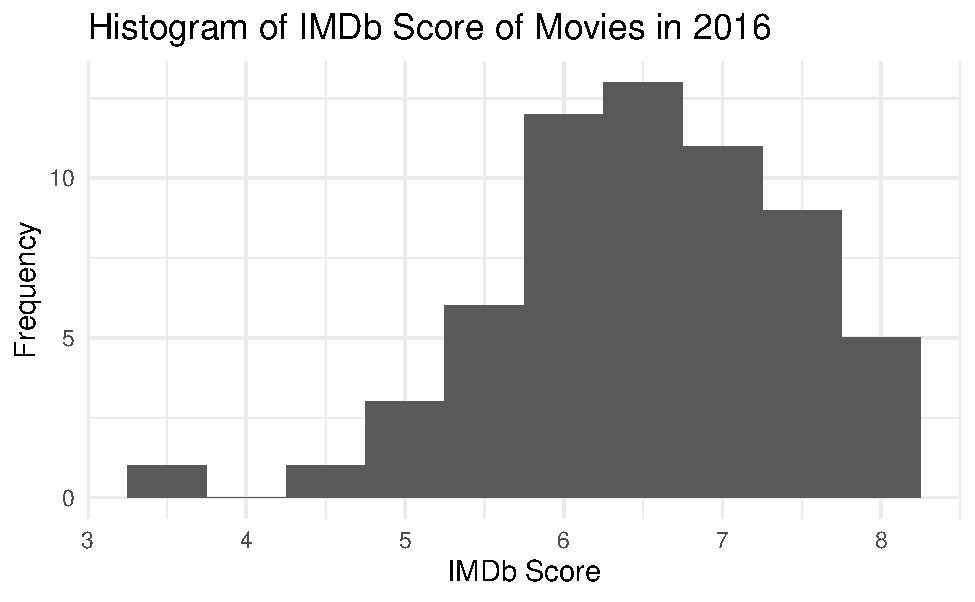
\includegraphics[width=0.7\linewidth]{04-EDA-quantitative_files/figure-latex/unnamed-chunk-3-1} \end{center}

\begin{enumerate}
\def\labelenumi{\arabic{enumi}.}
\setcounter{enumi}{7}
\tightlist
\item
  Which range of IMBb scores have the highest frequency?
\end{enumerate}

\vspace{0.5in}

\begin{enumerate}
\def\labelenumi{\arabic{enumi}.}
\setcounter{enumi}{8}
\tightlist
\item
  What is the shape of the distribution of IMDb scores?
\end{enumerate}

\vspace{0.5in}

The boxplot is created using the five number summary:

\begin{itemize}
\item
  Minimum value
\item
  Quartile 1 (Q1) - the value at the 25th percentile
\item
  Median - the value at the 50th percentile
\item
  Quartile 3 (Q3) - the value at the 75th percentile
\item
  Maximum value
\end{itemize}

\begin{enumerate}
\def\labelenumi{\arabic{enumi}.}
\setcounter{enumi}{9}
\tightlist
\item
  The three smallest IMDb scores in the data set are 3.4, 3.5, and 3.7 and the three largest IMDb scores are 8.5, 8.7, and 9.1. Using the summary statistics above, sketch a boxplot of IMDb Score. Be sure to label the axes.
\end{enumerate}

\vspace{2in}

\hypertarget{displaying-a-single-categorical-and-single-quantitative-variable}{%
\section{Displaying a Single Categorical and Single Quantitative Variable}\label{displaying-a-single-categorical-and-single-quantitative-variable}}

The boxplot of `Budget' in millions by `Content rating' is plotted using the code below. This plot helps to compare the budget for different levels of content rating.

\begin{center}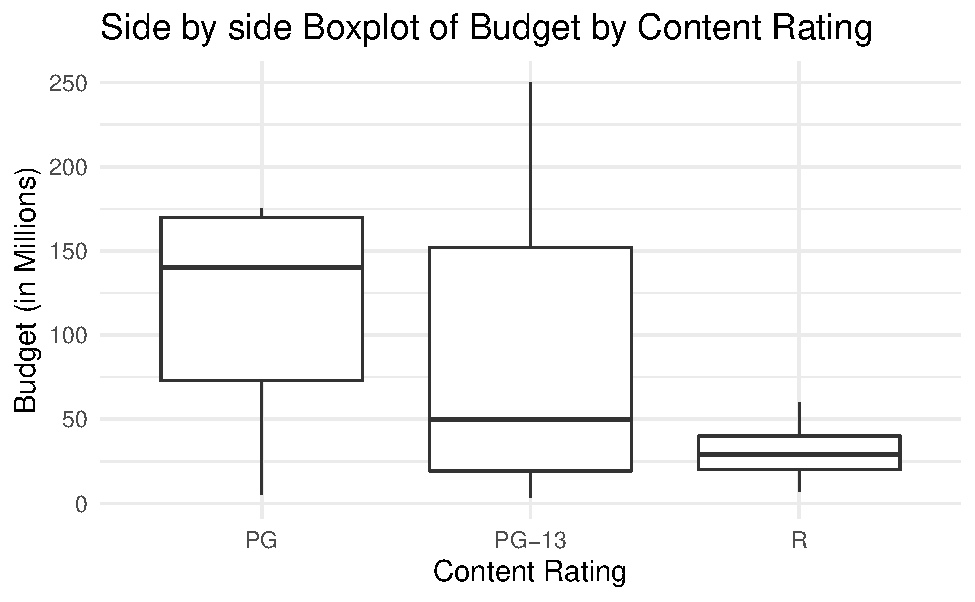
\includegraphics[width=0.7\linewidth]{04-EDA-quantitative_files/figure-latex/unnamed-chunk-4-1} \end{center}

\begin{enumerate}
\def\labelenumi{\arabic{enumi}.}
\setcounter{enumi}{10}
\tightlist
\item
  Answer the following questions about the boxplots above.
\end{enumerate}

\begin{enumerate}
\def\labelenumi{\alph{enumi}.}
\item
  Which content rating has the highest center?
  \vspace{0.5in}
\item
  Which content rating has the largest spread?
  \vspace{0.5in}
\item
  Which content rating is the most symmetric?
  \vspace{0.5in}
\item
  Fifty percent of movies in 2016 with a PG-13 content rating fall below what value?
  \vspace{0.5in}
\item
  What is the value for Q3 for the PG-13 rating? Interpret this value in context.
  \vspace{1in}
\end{enumerate}

\hypertarget{additional-notes}{%
\section{Additional Notes}\label{additional-notes}}

Use this space to summarize your thoughts and take additional notes on today's activity

\hypertarget{exploratory-data-analysis-multivariate-thinking}{%
\chapter{Exploratory Data Analysis: Multivariate Thinking}\label{exploratory-data-analysis-multivariate-thinking}}

\hypertarget{learning-objectives}{%
\section{Learning Objectives}\label{learning-objectives}}

\begin{itemize}
\item
  Identify and create appropriate summary statistics and plots
  given a data set with two quantitative variables
\item
  Use scatterplots to assess the relationship between two quantitative variables
\item
  Find the correlation coefficient
\item
  Find the estimated line of regression using summary statistics and R Linear Model Output
\item
  Understand what the slope coefficient represents
\item
  Understand what the coefficient of determination is
\end{itemize}

\hypertarget{movies-released-in-2016}{%
\section{Movies Released in 2016}\label{movies-released-in-2016}}

We will revisit the data set used last week collected on Movies released since 1916 to 2016. Here is a reminder of the variables collected on these movies.

\begin{itemize}
\item
  Year: Year the movie was released
\item
  Budget: The amount of money (in US \$ millions) budgeted for the production of the movie
\item
  Revenue: The amount of money (in US \$ millions) the movie made after release
\item
  Duration: The length of the movie (in minutes)
\item
  Content Rating: Rating of the movie (G, PG, PG-13, R, Not Rated)
\item
  IMDb Score: User rating score from 1 to 10
\item
  Genre: Category the movie falls into
\item
  Movie Facebook Likes: Number of likes a movie receives on Facebook
\end{itemize}

\hypertarget{terminology-review}{%
\section{Terminology Review}\label{terminology-review}}

In today's activity we will review summary measures and plots for two quantitative variables. Some terms covered in this activity are

\begin{itemize}
\item
  Scatterplot
\item
  Correlation
\item
  Slope
\item
  Line of Regression
\item
  Coefficient of determination
\end{itemize}

To review these concepts see Chapter 3 in the textbook.

\hypertarget{vocabulary-review}{%
\section{Vocabulary Review}\label{vocabulary-review}}

\begin{enumerate}
\def\labelenumi{\arabic{enumi}.}
\tightlist
\item
  What type of plot is used to display two quantitative variables?
\end{enumerate}

\vspace{0.5in}

\begin{enumerate}
\def\labelenumi{\arabic{enumi}.}
\setcounter{enumi}{1}
\tightlist
\item
  What summary statistics are used to describe the relationship between two quantitative variables?
\end{enumerate}

\vspace{0.5in}

We will look at the relationship between `Budget' and `Revenue' for movies released in 2016. This shows a scatterplot of `Budget' as a predictor of `Revenue' (note: both variables are measures in ``millions of dollars''.

\begin{Shaded}
\begin{Highlighting}[]
\KeywordTok{ggplot}\NormalTok{(}\DataTypeTok{data =}\NormalTok{ moviesa,   }\CommentTok{\#This is the data set}
       \KeywordTok{aes}\NormalTok{(}\DataTypeTok{x =}\NormalTok{ budget\_mil, }\DataTypeTok{y =}\NormalTok{ revenue\_mil))}\OperatorTok{+}\StringTok{  }\CommentTok{\#Specify variables}
\StringTok{  }\KeywordTok{geom\_point}\NormalTok{() }\OperatorTok{+}\StringTok{  }\CommentTok{\#Add scatterplot of points}
\StringTok{  }\KeywordTok{labs}\NormalTok{(}\DataTypeTok{x =} \StringTok{"Budget in Millions ($)"}\NormalTok{,  }\CommentTok{\#Label x{-}axis}
       \DataTypeTok{y =} \StringTok{"Revenue in Millions ($)"}\NormalTok{,  }\CommentTok{\#Label y{-}axis}
       \DataTypeTok{title =} \StringTok{"Revenue vs. Budget"}\NormalTok{) }\OperatorTok{+}\StringTok{ }\CommentTok{\#Be sure to tile your plots}
\StringTok{  }\KeywordTok{geom\_smooth}\NormalTok{(}\DataTypeTok{method =} \StringTok{"lm"}\NormalTok{, }\DataTypeTok{se =} \OtherTok{FALSE}\NormalTok{)  }\CommentTok{\#Add regression line}
\end{Highlighting}
\end{Shaded}

\begin{center}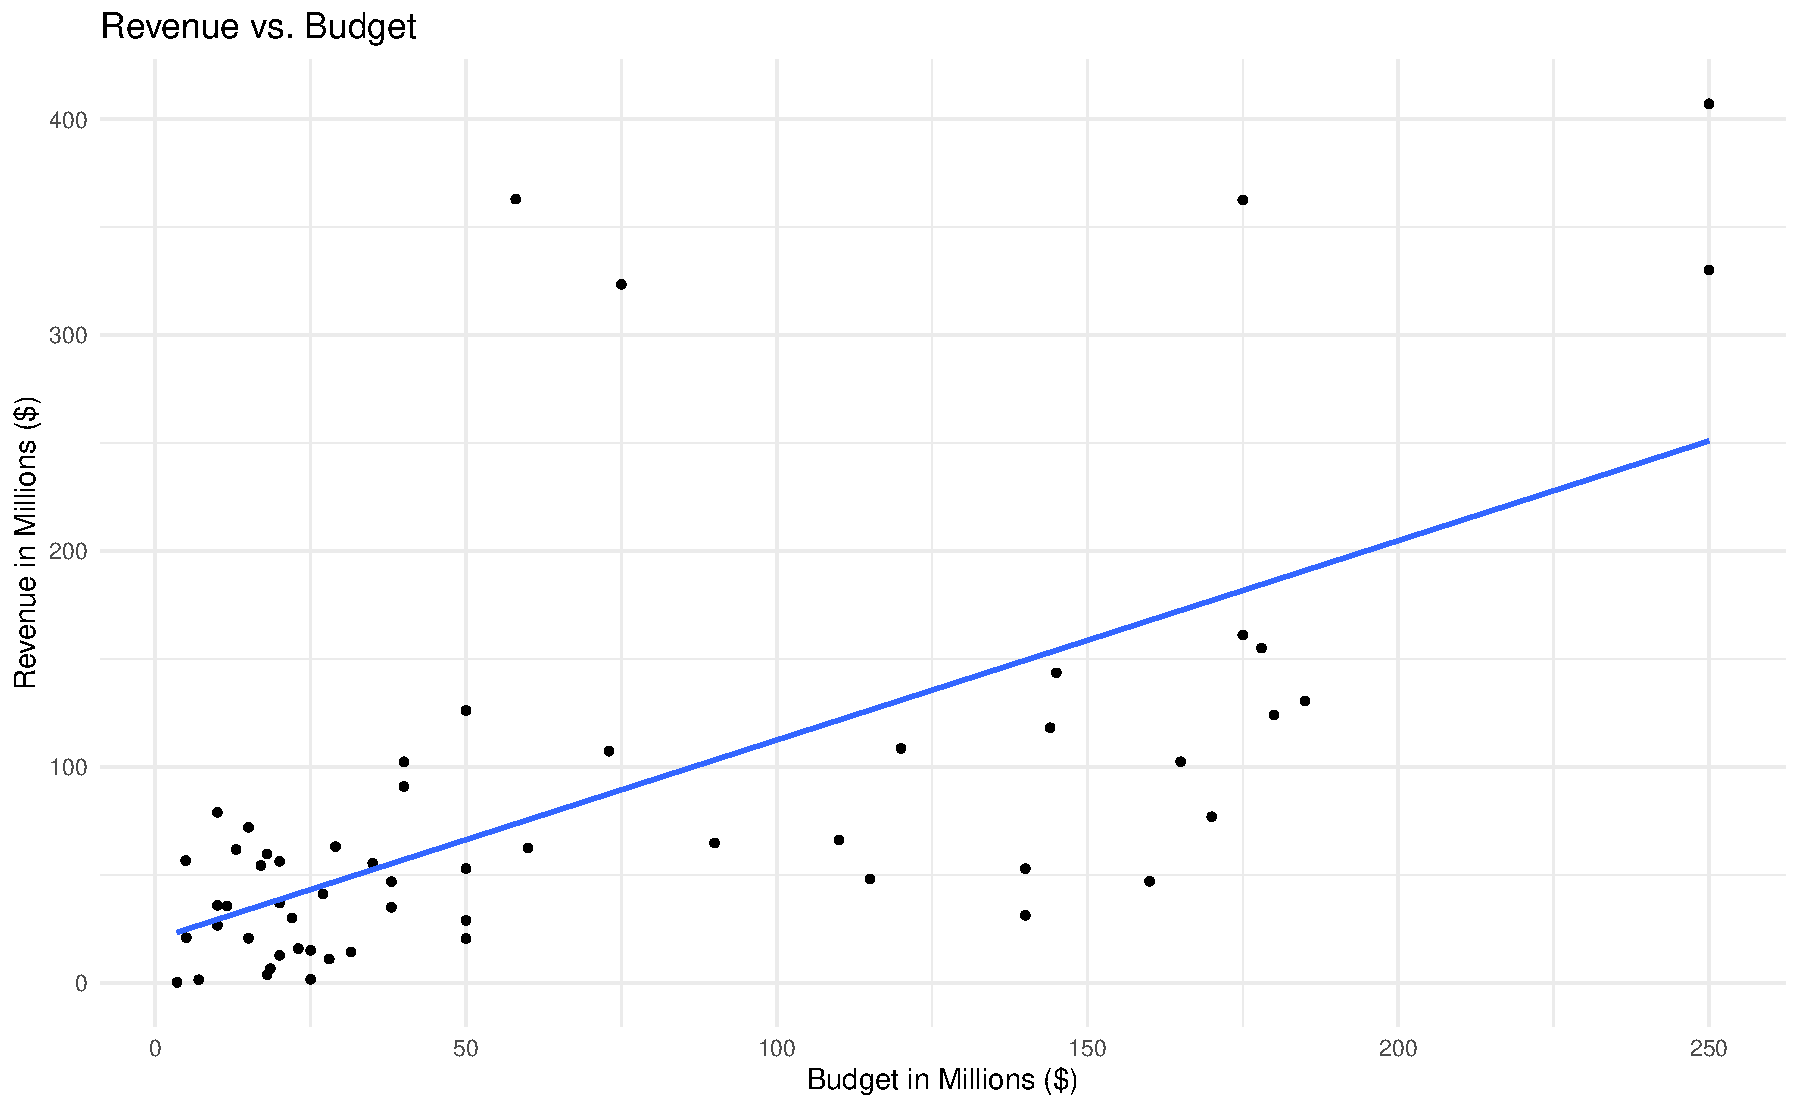
\includegraphics[width=0.7\linewidth]{05-EDA-multivariate_files/figure-latex/unnamed-chunk-2-1} \end{center}

\begin{enumerate}
\def\labelenumi{\arabic{enumi}.}
\setcounter{enumi}{2}
\item
  Assess the four features of the scatterplot that describe this relationship.

  \begin{itemize}
  \tightlist
  \item
    Form (linear, non-linear)
    \vspace{1in}
  \item
    Direction (positive, negative)
  \end{itemize}
\end{enumerate}

\vspace{1in}

\begin{itemize}
\tightlist
\item
  Strength
\end{itemize}

\vspace{1in}

\begin{itemize}
\tightlist
\item
  Unusual Observations or Outliers
\end{itemize}

\vspace{1in}

\begin{enumerate}
\def\labelenumi{\arabic{enumi}.}
\setcounter{enumi}{3}
\tightlist
\item
  Does there appear to be an association between `Budget' and `Revenue'? Explain.
\end{enumerate}

\vspace{1in}

\hypertarget{correlation}{%
\section{Correlation}\label{correlation}}

Correlation measures the strength and the direction between two quantitative variables. The closer the value of correlation to + or - 1 the stronger the linear relationship. Values close to zero indicate a very weak linear relationship between the two variables. The following output shows a correlation matrix between several pairs of quantitative variables.

\begin{verbatim}
#>                      budget_mil revenue_mil duration imdb_score
#> budget_mil               1.0000      0.6466   0.5274     0.3081
#> revenue_mil              0.6466      1.0000   0.2516     0.4876
#> duration                 0.5274      0.2516   1.0000     0.2362
#> imdb_score               0.3081      0.4876   0.2362     1.0000
#> movie_facebook_likes     0.6481      0.6710   0.5619     0.3462
#>                      movie_facebook_likes
#> budget_mil                         0.6481
#> revenue_mil                        0.6710
#> duration                           0.5619
#> imdb_score                         0.3462
#> movie_facebook_likes               1.0000
\end{verbatim}

\begin{enumerate}
\def\labelenumi{\arabic{enumi}.}
\setcounter{enumi}{4}
\tightlist
\item
  Using the output above, which two variables have the strongest correlation?
\end{enumerate}

\vspace{0.5in}

\begin{enumerate}
\def\labelenumi{\arabic{enumi}.}
\setcounter{enumi}{5}
\tightlist
\item
  What is the value of correlation between `Budget' and `Revenue'?
\end{enumerate}

\vspace{0.5in}

\begin{enumerate}
\def\labelenumi{\arabic{enumi}.}
\setcounter{enumi}{6}
\tightlist
\item
  Based on the value of correlation what would the sign of the slope be? Positive or negative? Explain.
\end{enumerate}

\vspace{1in}

\begin{enumerate}
\def\labelenumi{\arabic{enumi}.}
\setcounter{enumi}{7}
\tightlist
\item
  Does your answer to question 13 match the direction you choose in question 3?
\end{enumerate}

\vspace{0.5in}

\begin{enumerate}
\def\labelenumi{\arabic{enumi}.}
\setcounter{enumi}{8}
\tightlist
\item
  Explain why the correlation values on the diagonal are equal to 1.0.
\end{enumerate}

\vspace{1in}

\hypertarget{slope}{%
\section{Slope}\label{slope}}

The slope measures the change in y for each increase in x by 1. In other words, as the x variable increases by 1 unit, the y variable changes (increase/decreases) by the value of slope.

The linear model function in R gives us the summary for the least squares regression line. The estimate for (Intercept) is the y-intercept for the line of least squares and the estimate for budget is the value of \(b_1\), the slope.

\begin{verbatim}
#>               Estimate Std. Error  t value     Pr(>|t|)
#> (Intercept) 20.0362329 14.3458255 1.396659 1.677479e-01
#> budget_mil   0.9236972  0.1418579 6.511426 1.806269e-08
\end{verbatim}

\begin{enumerate}
\def\labelenumi{\arabic{enumi}.}
\setcounter{enumi}{9}
\tightlist
\item
  Write out the least squares line using the summary statistics provided.
\end{enumerate}

\vspace{1in}

\begin{enumerate}
\def\labelenumi{\arabic{enumi}.}
\setcounter{enumi}{10}
\tightlist
\item
  Interpret the value of slope in context of the problem.
\end{enumerate}

\vspace{1in}

\begin{enumerate}
\def\labelenumi{\arabic{enumi}.}
\setcounter{enumi}{11}
\tightlist
\item
  Using the least squares line from Question 10, predict the revenue for a movie with a budget of 165 million.
\end{enumerate}

\vspace{1in}

\hypertarget{residuals}{%
\section{Residuals:}\label{residuals}}

The model we are using assumes the relationship between the two variables follows a straight line. The residuals are the errors, or the part that hasn't been modeled by the line.

\begin{center}
Data = Model + Residual

Residual = Data - Model

$e_i=y_i-\hat{y}_i$
\end{center}

\begin{enumerate}
\def\labelenumi{\arabic{enumi}.}
\setcounter{enumi}{12}
\tightlist
\item
  The movie, \emph{Independence Day: Resurgence}, had a budget of 165 million and revenue of 102.315 million. Find the residual for this movie.
\end{enumerate}

\vspace{1in}

\begin{enumerate}
\def\labelenumi{\arabic{enumi}.}
\setcounter{enumi}{13}
\tightlist
\item
  Did the line of regression overestimate or underestimate the revenue for this movie?
\end{enumerate}

\vspace{1in}

\hypertarget{coefficient-of-determination}{%
\section{Coefficient of Determination}\label{coefficient-of-determination}}

The coefficient of determination, \(R^2\), can also be used to describe the strength of the linear relationship between two quantitative variables. \(R^2\) describes the amount of variation in the response that is explained by the least squares line with the explanatory variable.

\begin{enumerate}
\def\labelenumi{\arabic{enumi}.}
\setcounter{enumi}{14}
\tightlist
\item
  Calculate the coefficient of determination between `Budget' and `Revenue'.
\end{enumerate}

\vspace{1in}

\begin{enumerate}
\def\labelenumi{\arabic{enumi}.}
\setcounter{enumi}{15}
\tightlist
\item
  Interpret the coefficient of determination in context of the problem.
\end{enumerate}

\vspace{1in}

\hypertarget{multivariate-plot}{%
\section{Multivariate Plot}\label{multivariate-plot}}

In the next plot we are graphing three variables.

\begin{Shaded}
\begin{Highlighting}[]
\KeywordTok{ggplot}\NormalTok{(}\DataTypeTok{data =}\NormalTok{ moviesa,   }\CommentTok{\#This is the data set}
       \KeywordTok{aes}\NormalTok{(}\DataTypeTok{x =}\NormalTok{ budget\_mil, }\DataTypeTok{y =}\NormalTok{ revenue\_mil, }\DataTypeTok{color =}\NormalTok{ content\_rating))}\OperatorTok{+}\StringTok{  }\CommentTok{\#Specify variables}
\StringTok{  }\KeywordTok{geom\_point}\NormalTok{() }\OperatorTok{+}\StringTok{  }\CommentTok{\#Add scatterplot of points}
\StringTok{  }\KeywordTok{labs}\NormalTok{(}\DataTypeTok{x =} \StringTok{"Budget in Millions ($)"}\NormalTok{,  }\CommentTok{\#Label x{-}axis}
       \DataTypeTok{y =} \StringTok{"Revenue in Millions ($)"}\NormalTok{,  }\CommentTok{\#Label y{-}axis}
       \DataTypeTok{color =} \StringTok{"Content Rating"}\NormalTok{,  }\CommentTok{\#Label legend}
       \DataTypeTok{title =} \StringTok{"Revenue vs. Budget"}\NormalTok{) }\OperatorTok{+}\StringTok{ }\CommentTok{\#Be sure to tile your plots}
\StringTok{  }\KeywordTok{geom\_smooth}\NormalTok{(}\DataTypeTok{method =} \StringTok{"lm"}\NormalTok{, }\DataTypeTok{se =} \OtherTok{FALSE}\NormalTok{)  }\CommentTok{\#Add regression line}
\end{Highlighting}
\end{Shaded}

\begin{center}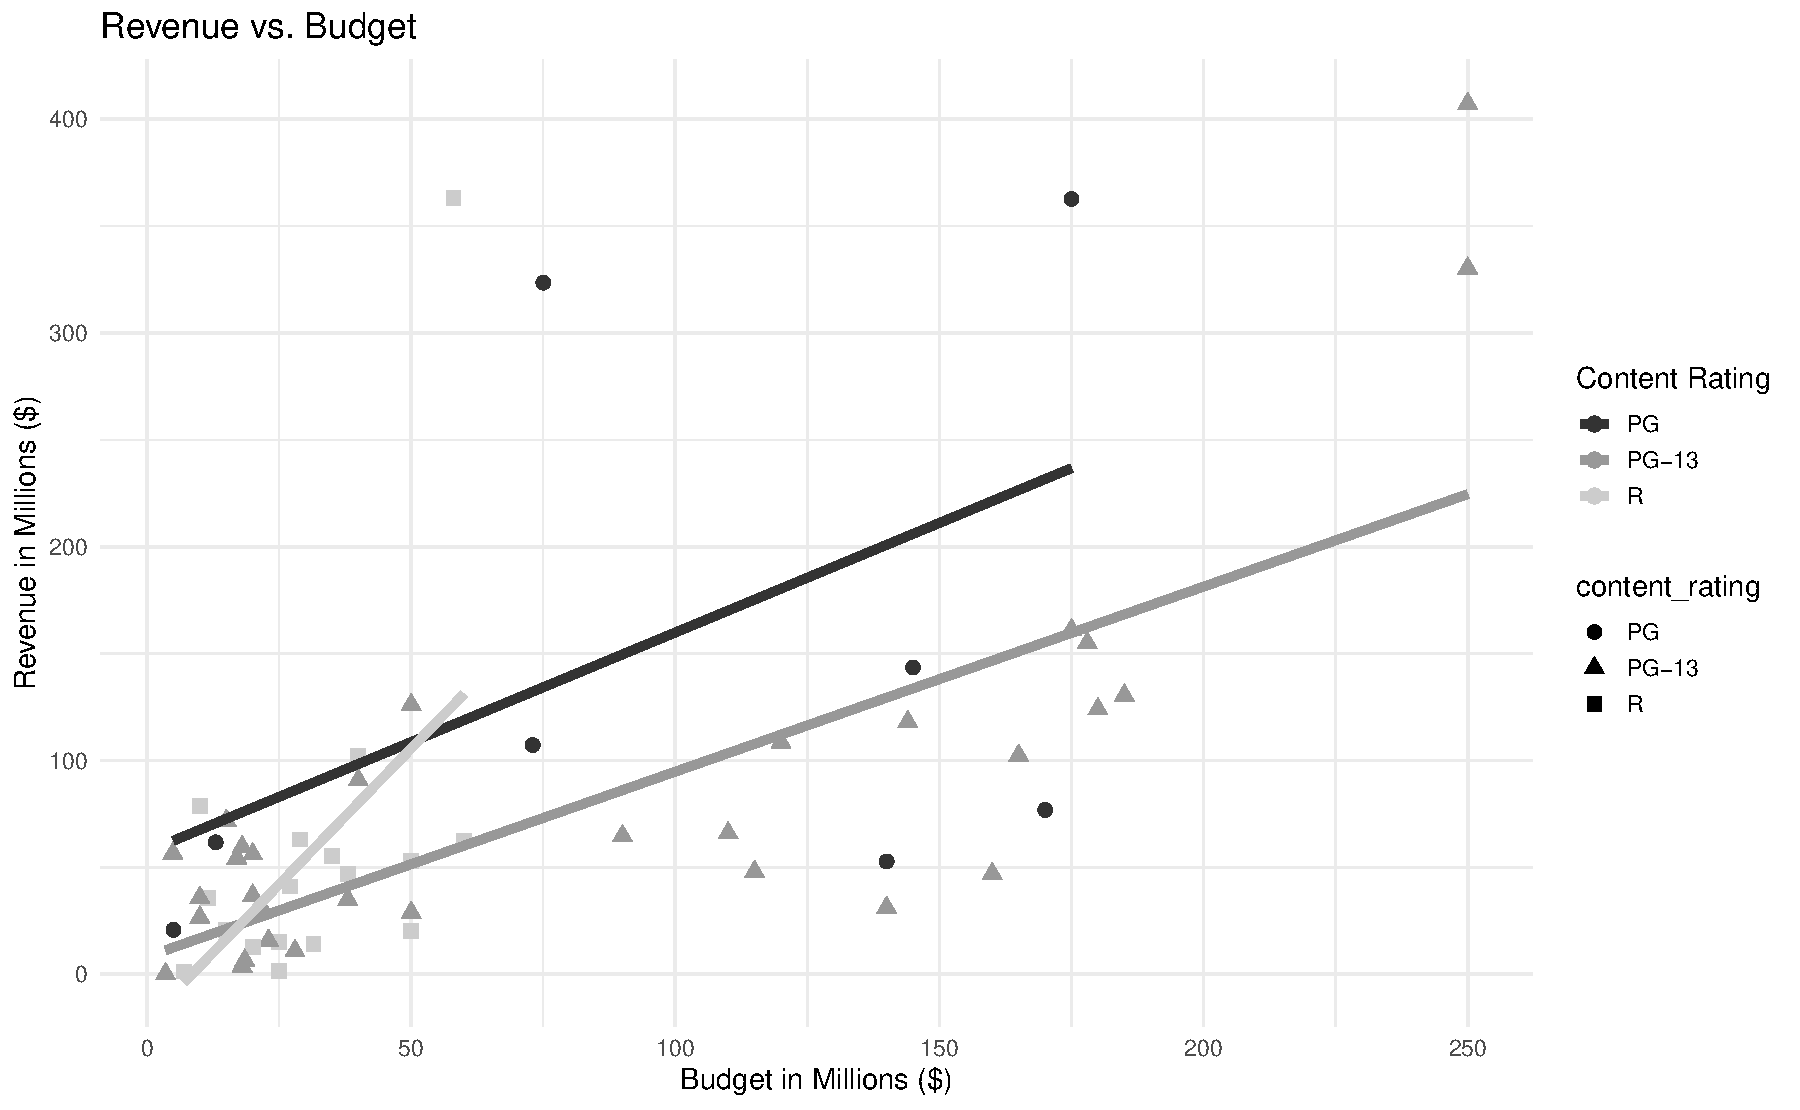
\includegraphics[width=0.7\linewidth]{05-EDA-multivariate_files/figure-latex/unnamed-chunk-5-1} \end{center}

\begin{enumerate}
\def\labelenumi{\arabic{enumi}.}
\setcounter{enumi}{24}
\tightlist
\item
  Identify the three varables plotted in this graph.
\end{enumerate}

\vspace{0.5in}

\begin{enumerate}
\def\labelenumi{\arabic{enumi}.}
\setcounter{enumi}{25}
\tightlist
\item
  Does the relationship between `Budget' and `Revenue' differ among the different content ratings? Explain.
\end{enumerate}

\vspace{1in}

\hypertarget{additional-notes}{%
\section{Additional Notes}\label{additional-notes}}

Use this space to summarize your thoughts and take additional notes on today's activity

\end{document}
